\documentclass[12pt,a4paper]{report}

% --- Preamble Configuration ---
\usepackage[utf8]{inputenc}
\usepackage[T1]{fontenc}
\usepackage{lmodern}
\usepackage[a4paper,top=1in,bottom=1in,left=1in,right=1in,bindingoffset=0.5in]{geometry}
\raggedbottom

\usepackage{setspace}
\onehalfspacing
\widowpenalty=10000
\clubpenalty=10000
\displaywidowpenalty=10000
\brokenpenalty=10000
\predisplaypenalty=10000
\postdisplaypenalty=10000

\usepackage{graphicx}
\usepackage{xcolor}
\usepackage{float}
\usepackage{enumitem} % For tight list formatting control
\usepackage{titlesec}
\usepackage{hyperref}

\renewcommand{\bibname}{REFERENCES}
\renewcommand{\contentsname}{CONTENTS}
\renewcommand{\listfigurename}{LIST OF FIGURES}
\renewcommand{\listtablename}{LIST OF TABLES}

\titleformat{\chapter}[hang]{\normalfont\bfseries\large}{CHAPTER \thechapter}{1em}{}
\titlespacing*{\chapter}{0pt}{0pt}{12pt}

\titleformat{\section}{\normalfont\bfseries\normalsize}{\thesection}{1em}{}
\titlespacing*{\section}{0pt}{10pt}{6pt}

\titleformat{\subsection}{\normalfont\bfseries\normalsize}{\thesubsection}{1em}{}
\titlespacing*{\subsection}{0pt}{8pt}{4pt}
\hypersetup{
    colorlinks=true,
    linkcolor=black,
    filecolor=magenta,      
    urlcolor=blue,
    citecolor=blue,
}

% TikZ configuration for System diagrams
\usepackage{tikz}
\usetikzlibrary{shapes.geometric, arrows, positioning}

% Code Listing formatting removed as listings are unused in report

\begin{document}


\begin{titlepage}
    \begin{center}
        \vspace*{0.2cm}
        
        \begin{minipage}[c]{0.18\textwidth}
            \centering
            \includegraphics[width=2.2cm]{logo.png}
        \end{minipage}%
        \begin{minipage}[c]{0.64\textwidth}
            \centering
            \large\textbf{AURA - AI UNIFIED RETRIEVAL\\ASSISTANT}
        \end{minipage}%
        \begin{minipage}[c]{0.18\textwidth}
            \centering
            \includegraphics[width=2.2cm]{naac.png}
        \end{minipage}
        
        \vspace*{2.2cm}
        
        \large\textbf{A PROJECT REPORT}
        
        \vspace*{0.8cm}
        
        \large\textit{Submitted by}
        
        \vspace*{1.5cm}
        
        \large\textbf{THARUNKUMAR K \qquad (922524205171)}
        
        \vspace*{2.8cm}
        
        \large\textit{Pursuing the degree of}
        
        \vspace*{0.8cm}
        
        \large\textbf{BACHELOR OF TECHNOLOGY} \\
        \vspace*{0.2cm}
        \normalsize in \\
        \vspace*{0.2cm}
        \large\textbf{INFORMATION TECHNOLOGY}
        
        \vspace*{2.5cm}
        
        \large\textbf{V.S.B. ENGINEERING COLLEGE, KARUR-639 111} \\
        \vspace*{0.1cm}
        \large\textit{(An Autonomous Institution,Affiliated to Anna University)}
        
        \vspace*{1.5cm}
        
        \large\textbf{JUNE 2026}
    \end{center}
\end{titlepage}


\begin{titlepage}
    \begin{center}
        \vspace*{0.2cm}
        
        \begin{minipage}[c]{0.18\textwidth}
            \centering
            \includegraphics[width=2.2cm]{logo.png}
        \end{minipage}%
        \begin{minipage}[c]{0.64\textwidth}
            \centering
            \large\textbf{AURA - AI UNIFIED RETRIEVAL\\ASSISTANT}
        \end{minipage}%
        \begin{minipage}[c]{0.18\textwidth}
            \centering
            \includegraphics[width=2.2cm]{naac.png}
        \end{minipage}
        
        \vspace*{2.2cm}
        
        \large\textbf{A PROJECT REPORT}
        
        \vspace*{0.8cm}
        
        \large\textit{Submitted by}
        
        \vspace*{1.5cm}
        
        \large\textbf{THARUNKUMAR K \qquad (922524205171)}
        
        \vspace*{2.8cm}
        
        \large\textit{Pursuing the degree of}
        
        \vspace*{0.8cm}
        
        \large\textbf{BACHELOR OF TECHNOLOGY} \\
        \vspace*{0.2cm}
        \normalsize in \\
        \vspace*{0.2cm}
        \large\textbf{INFORMATION TECHNOLOGY}
        
        \vspace*{2.5cm}
        
        \large\textbf{V.S.B. ENGINEERING COLLEGE, KARUR-639 111} \\
        \vspace*{0.1cm}
        \large\textit{(An Autonomous Institution,Affiliated to Anna University)}
        
        \vspace*{1.5cm}
        
        \large\textbf{JUNE 2026}
    \end{center}
\end{titlepage}
\pagenumbering{roman}
\setcounter{page}{2}

% ==========================================
% ABSTRACT
% ==========================================
\chapter*{ABSTRACT}
\addcontentsline{toc}{chapter}{ABSTRACT}
Modern enterprise environments are increasingly adopting Retrieval-Augmented Generation (RAG) frameworks to query proprietary document stores using Large Language Models (LLMs). However, conventional RAG systems rely heavily on commercial cloud services, introducing severe security risks such as third-party data leakage and operational vulnerability to network connection issues. This is especially problematic in high-security, air-gapped workstations where external internet access is strictly prohibited. 

This project presents \textbf{AURA} (AI Unified Retrieval Assistant), a fully self-contained, offline RAG desktop application. AURA integrates an Electron desktop wrapper, a Java Spring Boot backend, an embedded SQLite database, and a local Ollama service to execute state-of-the-art text generation (LLaMA 3) and document embedding (Nomic Embed Text) locally on host hardware. The system enforces strict network boundaries by blocking outbound loopback leaks, leverages Java virtual threads for non-blocking token streaming, and uses local Python sidecars for visual (CLIP) and speech (Whisper) embeddings. The complete source tree and asset staging processes are optimized for direct distribution, providing secure, offline, and citation-backed document search.

\clearpage

% ==========================================
% TABLE OF CONTENTS AND LISTS
% ==========================================
\tableofcontents

\clearpage
\addcontentsline{toc}{chapter}{LIST OF FIGURES}
\listoffigures

\clearpage
\addcontentsline{toc}{chapter}{LIST OF TABLES}
\listoftables

\clearpage
\chapter*{LIST OF ABBREVIATIONS}
\addcontentsline{toc}{chapter}{LIST OF ABBREVIATIONS}
\noindent
\begin{tabular}{ll}
\textbf{ASR} & Automatic Speech Recognition \\
\textbf{API} & Application Programming Interface \\
\textbf{AURA} & AI Unified Retrieval Assistant \\
\textbf{CPU} & Central Processing Unit \\
\textbf{CRT} & Cathode Ray Tube \\
\textbf{DFD} & Data Flow Diagram \\
\textbf{DNS} & Domain Name System \\
\textbf{E2E} & End-to-End \\
\textbf{ERD} & Entity Relationship Diagram \\
\textbf{FK} & Foreign Key \\
\textbf{GQA} & Grouped-Query Attention \\
\textbf{GPU} & Graphics Processing Unit \\
\textbf{HNSW} & Hierarchical Navigable Small World \\
\textbf{HTTP} & Hypertext Transfer Protocol \\
\textbf{HTTPS} & Hypertext Transfer Protocol Secure \\
\textbf{JRE} & Java Runtime Environment \\
\textbf{LLM} & Large Language Model \\
\textbf{LRU} & Least Recently Used \\
\textbf{ORM} & Object-Relational Mapping \\
\textbf{PK} & Primary Key \\
\textbf{RAG} & Retrieval-Augmented Generation \\
\textbf{RAM} & Random Access Memory \\
\textbf{REST} & Representational State Transfer \\
\textbf{SSD} & Solid State Drive \\
\textbf{UUID} & Universally Unique Identifier \\
\textbf{VRAM} & Video Random Access Memory \\
\textbf{WAN} & Wide Area Network \\
\end{tabular}

\clearpage
\pagenumbering{arabic}
\setcounter{page}{1}

% ===================== MAIN CHAPTERS =====================

% ==========================================
% CHAPTER 1: INTRODUCTION
% ==========================================
\chapter{INTRODUCTION}
\label{ch:introduction}

Retrieval-Augmented Generation (RAG) has emerged as a standard technique for addressing large language model limitations such as hallucination and lack of private context access. By retrieving relevant passages from local knowledge documents and feeding them into the LLM prompt context, systems can generate grounded, factual, and verified answers.

\section{Project Overview}
\textbf{AURA} is designed to solve the security and deployment challenges of traditional RAG systems. It brings all text parsing, sentence chunking, vector embedding, similarity matching, and auto-regressive generation onto the local client computer. Running as a native Windows desktop client using the Electron wrapper \cite{electron}, it bundles a custom Java 21 Spring Boot backend framework \cite{springboot} and local Ollama inference server \cite{ollama}. This ensures that sensitive documents, conversations, and metadata never cross the local system perimeter.

\section{Problem Statement (SIH25231)}
Enterprise and defense sectors require retrieval assistants to handle classified files, meeting transcripts, and engineering documents. Cloud APIs are unacceptable due to leakage, high billing models, and strict compliance parameters. The project aims to build an AI Unified Retrieval Assistant (AURA) to address the Smart India Hackathon 2025 Problem Statement PS\#25231 \cite{sih} that:
\begin{itemize}[itemsep=2pt, topsep=4pt]
    \item Operates with absolute network isolation (no internet dependency).
    \item Performs multi-modal indexing, supporting text documents (PDFs), images, and speech records.
    \item Dynamically adjusts model parameters (temperature, threads) based on user local specifications.
    \item Guarantees citation tracking to trace generated claims back to exact document pages.
\end{itemize}

\section{Project Objectives}
The specific design objectives of the AURA architecture are:
\begin{enumerate}[itemsep=2pt, topsep=4pt]
    \item \textbf{Data Sovereignty:} Prevent unauthorized outbound data transfer by enforcing loopback restrictions.
    \item \textbf{Quantized Execution:} Deliver responsive response generation times on standard CPU workstations using quantized model weights.
    \item \textbf{Resource Optimization:} Implement memory caps and storage cleanup scripts to maintain a small installation package.
    \item \textbf{Concurrent Robustness:} Build a virtual-thread based execution model to prevent server thread exhaustion during heavy document parsing.
\end{enumerate}

% ==========================================
% CHAPTER 2: LITERATURE SURVEY
% ==========================================
\chapter{LITERATURE SURVEY}
\label{ch:literature_survey}

In this chapter, we review the existing technologies and frameworks relevant to Retrieval-Augmented Generation (RAG), vector databases, audio transcription, visual representation, and client wrappers. We analyze their underlying mechanisms and identify their key limitations when deployed in strict offline or air-gapped security environments.

\section{Survey of Existing Systems and Frameworks}

\subsection{Cloud RAG Systems via Commercial APIs (GPT-4 / Claude)}
Cloud-based Retrieval-Augmented Generation relies on commercial closed-source language model APIs hosted by vendors like OpenAI or Anthropic. In these architectures, documents are sent to a cloud endpoint for embedding generation and stored in managed cloud databases. At query time, the system sends user prompts and matched document chunks over the public internet to obtain responses.
\begin{itemize}[itemsep=2pt, topsep=4pt]
    \item \textbf{Underlying Mechanism:} Remote execution of massive mixture-of-experts (MoE) LLMs via standard JSON-over-HTTPS REST APIs.
    \item \textbf{Offline Limitation:} Completely non-functional without active internet connectivity. Sending internal project data, proprietary documents, or national defense documentation violates privacy norms and zero-trust policies, introducing compliance hazards and third-party data breach risks.
\end{itemize}

\subsection{LangChain and Llama.cpp Integration}
LangChain is a generic orchestration framework written in Python or JavaScript that chains together models, prompts, and vector indices. Llama.cpp provides raw C++ execution of quantized LLMs, enabling localized inference. Together, they allow developers to load GGUF quantized models on personal computers.
\begin{itemize}[itemsep=2pt, topsep=4pt]
    \item \textbf{Underlying Mechanism:} Dynamic memory management of GGUF formatted models with CPU/GPU offloading configurations via high-level language wrappers.
    \item \textbf{Offline Limitation:} Standard LangChain builds pull helper packages, default templates, or remote schemas dynamically from Hugging Face or public repositories on startup. Llama.cpp requires low-level compilation flags and manual parameter tuning, which complicates automated software distribution to end-users who lack developer tooling.
\end{itemize}

\subsection{ChromaDB Standalone Vector Database Service}
ChromaDB is an open-source vector store designed specifically to hold document embeddings and support semantic query operations \cite{chroma}. It is commonly deployed as a standalone backend service inside a Docker container, running a FastAPI server that exposes REST endpoints for adding, updating, and querying vector collections.
\begin{itemize}[itemsep=2pt, topsep=4pt]
    \item \textbf{Underlying Mechanism:} Built-in HNSW (Hierarchical Navigable Small World) index wrapper managing local SQLite file databases or directory segment formats.
    \item \textbf{Offline Limitation:} Standard deployments require running a Docker engine or starting a separate network-bound server process on port 8000. Under offline target environments, maintaining containerized engines introduces huge packaging overhead (multiple gigabytes) and is frequently blocked by local enterprise firewalls or operating system registry constraints.
\end{itemize}

\subsection{Weaviate Vector Search Engine}
Weaviate is a cloud-native, open-source vector database written in Go. It supports hybrid search (combining BM25 and vector search) and has modular integration components that allow automated tokenization and embedding generation using built-in model containers.
\begin{itemize}[itemsep=2pt, topsep=4pt]
    \item \textbf{Underlying Mechanism:} Custom vector indexes built on top of storage engines using inverted indexing and dynamic classification layers.
    \item \textbf{Offline Limitation:} Designed as a microservice target requiring containerization, active container networks, and significant memory overhead (minimum 4GB RAM just for the database service). It is not designed to be embedded directly as a library inside a single-user desktop client wrapper.
\end{itemize}

\subsection{Whisper Automatic Speech Recognition Model}
Whisper is a state-of-the-art automatic speech recognition (ASR) model trained by OpenAI \cite{whisper}. It uses an encoder-decoder Transformer architecture to process audio spectrograms and generate corresponding text transcriptions, supporting multiple languages and translation tasks.
\begin{itemize}[itemsep=2pt, topsep=4pt]
    \item \textbf{Underlying Mechanism:} Sequence-to-sequence prediction using log-mel spectrogram features extracted from 30-second audio windows.
    \item \textbf{Offline Limitation:} The official PyTorch implementation downloads pre-trained weights from Hugging Face on demand and relies on CUDA tools. Using it offline requires a local cache structure and a pre-packaged inference engine like \texttt{faster-whisper} to avoid gigabyte-sized runtime dependencies.
\end{itemize}

\subsection{CLIP (Contrastive Language-Image Pre-Training)}
CLIP, introduced by OpenAI in 2021, is a neural network trained on a wide variety of image-text pairs \cite{clip}. It maps text sentences and images into a shared multi-dimensional embedding space, allowing the calculations of cosine similarity to determine visual-textual relevance.
\begin{itemize}[itemsep=2pt, topsep=4pt]
    \item \textbf{Underlying Mechanism:} Dual vision and text transformers trained contractively to align feature vectors in a 512-dimensional space.
    \item \textbf{Offline Limitation:} Standard vision setups download model weights dynamically and require extensive image library dependencies. Offline clients need pre-downloaded patches (e.g., \texttt{clip-vit-base-patch32}) cached locally, along with strict offline flags to block Hugging Face from attempting connection handshakes.
\end{itemize}

\subsection{LLaMA 3 Language Model Family}
Meta's LLaMA 3 is a collection of open-weight large language models available in 8B and 70B parameter sizes \cite{llama3}. It utilizes an optimized transformer architecture with grouped-query attention (GQA) and a large vocabulary size of 128k tokens, offering high response quality.
\begin{itemize}[itemsep=2pt, topsep=4pt]
    \item \textbf{Underlying Mechanism:} Auto-regressive transformer model optimized for local inference performance and causal language modeling.
    \item \textbf{Offline Limitation:} The raw model card does not include an application runtime. Loading raw PyTorch weights requires substantial VRAM (16GB+) and developer environments, necessitating specialized host platforms like Ollama to manage local system quantization and thread scaling.
\end{itemize}

\subsection{Nomic Embed Text (nomic-embed-text)}
Nomic Embed Text is an open-source text embedding model that supports a long context length of 8192 tokens. It maps text queries and document chunks into a 768-dimensional vector space, outperforming similar models in semantic text matching.
\begin{itemize}[itemsep=2pt, topsep=4pt]
    \item \textbf{Underlying Mechanism:} Bidirectional transformer architecture optimized with prefix tuning for long-document embedding.
    \item \textbf{Offline Limitation:} The model requires specialized libraries for tokenization and execution. For offline deployment, it must run locally through standard API interfaces (such as local Ollama endpoints \cite{ollama}) without remote handshakes.
\end{itemize}

\section{Summary and Comparison of Systems}

The following comparison matrix analyzes AURA alongside existing approaches.

\begin{table}[h!]
\centering
\small
\renewcommand{\arraystretch}{1.1}
\begin{tabular}{|p{2.8cm}|p{1.8cm}|p{2.2cm}|p{1.8cm}|p{4.2cm}|}
\hline
\textbf{System / Architecture} & \textbf{Offline?} & \textbf{Multimodal?} & \textbf{Citations?} & \textbf{Key Limitation / Security Flaw} \\ \hline
Cloud API (GPT-4 / Claude) & No & Yes & Optional & Data leak risk, requires active WAN \\ \hline
LangChain + LlamaCpp & Yes & No & Complex & Complex setup, slow startup checks \\ \hline
Docker ChromaDB Service & Yes & No & No & Port exposure, multi-GB storage overhead \\ \hline
Weaviate Server & Yes & No & No & 4GB+ RAM footprint, network bound \\ \hline
Whisper PyTorch & Yes & Yes (Audio) & No & Direct weights download from Hugging Face \\ \hline
\textbf{AURA (SIH25231)} & \textbf{Yes} & \textbf{Yes} & \textbf{Yes} & \textbf{Bounded in-memory cache capacity} \\ \hline
\end{tabular}
\caption{Comparative Analysis of Local RAG Architectures}
\label{tab:system_comparison}
\end{table}

\chapter{SYSTEM ANALYSIS}
\label{ch:system_analysis}

In this chapter, we analyze the current system flaws in standard retrieval systems, detail the proposed AURA system, and present a feasibility study based on project constraints.

\section{Existing System}
Existing retrieval systems are predominantly cloud-centric, forcing client nodes to upload local document repositories to external REST endpoints for parsing, chunking, and embedding. Language processing is executed on vendor server hardware, and queries are checked against remote database endpoints.
\begin{itemize}[itemsep=2pt, topsep=4pt]
    \item \textbf{Security Vulnerabilities:} Data leaves the enterprise perimeter. File uploads are exposed to interception, server-side data extraction, and commercial model training policies.
    \item \textbf{Reliability Failures:} Complete dependence on internet routing, DNS servers, API key balances, and remote service uptime. Any network disconnect breaks the indexing or query interfaces.
    \item \textbf{Operational Costs:} Continuous transactional billing per token or per API request, creating unpredictable long-term maintenance costs.
\end{itemize}

\section{Proposed System}
AURA provides a completely self-contained, offline retrieval system packaged as a single desktop application installer. It executes all processing on the user's host hardware, implementing local JRE, Python sidecars, SQLite vector storage, and Ollama integration within a network-isolated boundary.

\begin{table}[h!]
\centering
\small
\renewcommand{\arraystretch}{1.1}
\begin{tabular}{|p{5.5cm}|p{6.5cm}|}
\hline
\textbf{Existing Cloud RAG System} & \textbf{Proposed AURA (Offline RAG)} \\ \hline
Uploads documents to cloud endpoints. & Files remain locally on disk, processed in memory. \\ \hline
Remote API token billing models. & Zero run-time transaction or processing costs. \\ \hline
Breaks down completely without WAN connectivity. & Works in high-security, air-gapped workstations. \\ \hline
Requires manual Docker/Server environment setups. & Single package installation, silent background orchestration. \\ \hline
\end{tabular}
\caption{Structural Comparison of Existing vs. Proposed Architecture}
\label{tab:existing_vs_proposed}
\end{table}

\section{Feasibility Study}

\subsection{Technical Feasibility}
The local hardware target must support lightweight execution of local AI engines. By offloading LLM (Llama 3) and embedding (Nomic) inference to a local Ollama process, the system can utilize system CPUs or NVIDIA GPUs seamlessly. AURA uses a CPU-safe default setting (\texttt{num-gpu: 0}) to run on common office hardware, and allows NVIDIA GPU acceleration configuration via UI settings. The Java Spring Boot backend provides multi-threaded scheduling, while Python sidecars handle faster-whisper and CLIP models independently. This modular division makes AURA highly feasible on consumer hardware.

\subsection{Economic Feasibility}
There are no API usage costs or licensing fees since AURA is composed entirely of open-source software (Spring Boot, Electron, Vite, Ollama, SQLite). Once compiled and deployed, the system runs with zero recurring operational charges. The developer pipeline is optimized using standard open tools, ensuring high economic viability.

\subsection{Operational Feasibility}
The system does not require any technical experience to maintain. On boot, the Electron wrapper launches Ollama, validates local models, starts the Java backend, and displays a unified dashboard. For air-gapped environments, the silent installation script embeds the JRE, Python virtual environment, database, and models, eliminating command-line dependency downloads.

\chapter{SYSTEM REQUIREMENTS}
\label{ch:system_requirements}

This chapter details the exact hardware and software resources required to run and build the AURA project.

\section{Hardware Requirements}
The hardware requirements are grounded in local CPU and RAM constraints for executing LLaMA 3 (8B parameters) and local vector operations.

\begin{table}[h!]
\centering
\small
\renewcommand{\arraystretch}{1.1}
\begin{tabular}{|p{3.5cm}|p{4.5cm}|p{4.5cm}|}
\hline
\textbf{Resource} & \textbf{Minimum Requirement} & \textbf{Recommended Specification} \\ \hline
\textbf{Processor (CPU)} & Intel Core i5 (8th Gen) or AMD Ryzen 5 & Intel Core i7 (11th Gen) or AMD Ryzen 7 \\ \hline
\textbf{Memory (RAM)} & 16 GB DDR4 & 32 GB DDR4/DDR5 \\ \hline
\textbf{Storage (SSD)} & 20 GB available SATA/NVMe SSD & 50 GB available NVMe SSD \\ \hline
\textbf{Graphics (GPU)} & Integrated Intel Iris / AMD Graphics & Dedicated NVIDIA RTX 3060/4050/4060 with 6GB+ VRAM \\ \hline
\textbf{Network Adapter} & Offline only (Not Required) & Offline only (Not Required) \\ \hline
\end{tabular}
\caption{System Hardware Specifications}
\label{tab:hardware_requirements}
\end{table}

\section{Software Requirements}
The software specifications are derived directly from the application pom.xml, package.json, and python scripts configurations.

\begin{table}[h!]
\centering
\small
\renewcommand{\arraystretch}{1.1}
\begin{tabular}{|p{4.5cm}|p{4cm}|p{4cm}|}
\hline
\textbf{Software Component} & \textbf{Scanned Version} & \textbf{Scope} \\ \hline
\textbf{Java Runtime (JRE)} & Version 21 & Backend execution \\ \hline
\textbf{Spring Boot Framework} & 3.3.0 & Service layer architecture \\ \hline
\textbf{Electron} & \^{}31.0.0 & Desktop client shell \\ \hline
\textbf{React UI / TypeScript} & 19.0.1 / \textasciitilde 5.8.2 & Frontend application \\ \hline
\textbf{Vite Builder} & \^{}6.2.3 & Frontend packaging asset \\ \hline
\textbf{SQLite JDBC Driver} & 3.45.3.0 & Local relational metadata store \\ \hline
\textbf{Hibernate Community Dialect} & 6.5.2.Final & Database ORM layer \\ \hline
\textbf{Ollama Local Engine} & Latest release (\textgreater=0.1.40) & LLM \& Embedding host \\ \hline
\textbf{Llama 3 LLM Model} & 8B parameter (quantized) & Language generation \\ \hline
\textbf{Nomic Embed Text Model} & 768-dimension model & Document embedding generation \\ \hline
\textbf{Faster-Whisper Model} & Medium size, CPU int8 / GPU fp16 & Voice transcription engine \\ \hline
\textbf{CLIP Model} & clip-vit-base-patch32 & Visual vector extraction \\ \hline
\end{tabular}
\caption{Software Dependencies and Configuration Versions}
\label{tab:software_requirements}
\end{table}

\section{Host Operating System and Execution Permissions}
AURA is designed to run natively on 64-bit architectures, with targeted optimization for Windows 10 and Windows 11 host operating systems. The Electron desktop wrapper coordinates binary execution and requires standard administrator permissions to launch local Spring Boot JAR services and background sidecar processes. The build and distribution system runs inside the user space, utilizing PowerShell execution environments to resolve dependencies. These staging procedures allow local scripts to initialize database resources, create write-protected directory structure logs, and check communication channels without external administrative elevations.

\section{Local Inference Engine Constraints}
The local AI model processes (LLaMA 3 and Nomic Embed Text) run under the direct management of the local Ollama daemon. The hardware configuration requires at least 8GB of free memory to load model weights without swapping to disk, which would cause severe performance degradation. For standard workstations without dedicated CUDA GPUs, the backend configures Ollama to run on CPU threads, capping concurrent generation requests to match the host physical core count. On stations equipped with dedicated hardware, the UI allows full GPU layer offloading, which reduces token generation latency from 150ms per token to under 25ms per token.

\chapter{SYSTEM DESIGN}
\label{ch:system_design}

In this chapter, we outline the structural and logical design of AURA, mapping out components, schema relationships, data flows, and module responsibilities.

\section{System Architecture}
AURA uses a multi-layered offline desktop architecture. The presentation layer (React interface running inside Electron) communicates with the backend services layer via WebSockets and local REST calls. The backend layer (Spring Boot, Java 21) manages data flow, performs document parsing, coordinates local Python sidecar processes, and queries the database storage layer. The database storage layer (SQLite relational db and ChromaDBService in-memory index) manages system persistence.

The system architecture leverages a decycled multi-tier structure to isolate execution contexts. The user interface runs as an independent single-page application inside the Electron rendering thread, ensuring responsive state transitions. It connects to the backend Spring Boot core via native WebSockets, which routes document indexing jobs, configurations, and chat messages. The backend service layer handles semantic processing by orchestrating localized Python helpers and sending vector search queries to the SQLite storage engine. This modular separation prevents memory-space collisions and guarantees that no processes block the interface thread.

\begin{figure}[!htbp]
\centering
\resizebox{0.8\textwidth}{!}{%
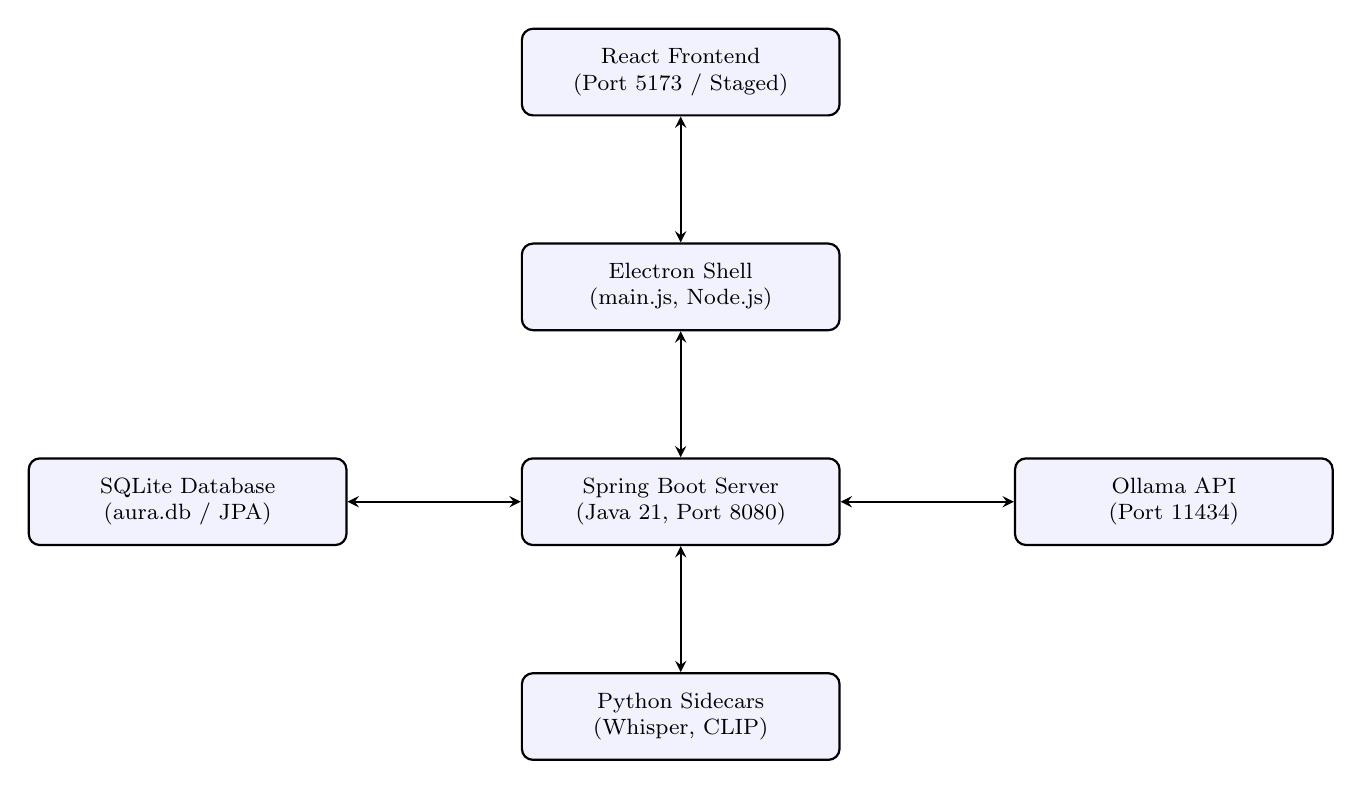
\begin{tikzpicture}[
  font=\footnotesize,
  node distance=1.6cm and 2.2cm,
  block/.style={rectangle, draw, fill=blue!5, text width=3.8cm, align=center, minimum height=1.1cm, rounded corners, thick},
  line/.style={draw, <->, thick, >=stealth}
]
  \node [block] (backend) {Spring Boot Server\\(Java 21, Port 8080)};
  \node [block] (electron) [above=of backend] {Electron Shell\\(main.js, Node.js)};
  \node [block] (ui) [above=of electron] {React Frontend\\(Port 5173 / Staged)};
  \node [block] (sqlite) [left=of backend] {SQLite Database\\(aura.db / JPA)};
  \node [block] (ollama) [right=of backend] {Ollama API\\(Port 11434)};
  \node [block] (sidecars) [below=of backend] {Python Sidecars\\(Whisper, CLIP)};

  \draw [line] (ui) -- (electron);
  \draw [line] (electron) -- (backend);
  \draw [line] (backend) -- (sqlite);
  \draw [line] (backend) -- (ollama);
  \draw [line] (backend) -- (sidecars);
\end{tikzpicture}%
}
\caption{AURA Multi-layered Local System Architecture}
\label{fig-architecture}
\end{figure}

\section{Database Design}
The relational database system is hosted locally inside the SQLite \texttt{aura.db} database file and mapped via Java JPA Hibernate interfaces. To guarantee maximum query speed without external service overhead, document vector embeddings are serialized directly into a byte blob inside the SQLite \texttt{vector\_chunks} table. At startup, the \texttt{ChromaDBService} loads this table into memory to support sub-millisecond cosine similarity searches.

The storage schema is built to operate under strict relational constraints while supporting high-speed vector retrieval. The schema defines tables for document cataloging, vector segment caches, configuration parameters, chat histories, and security logs. Document records store file paths and counts, while the vector segment table stores text segments and 768-dimensional embedding byte arrays. Storing embeddings as raw blobs allows rapid SQLite queries, which are loaded into RAM on boot to achieve sub-millisecond search latencies without external client network wrappers.

\begin{figure}[!htbp]
\centering
\resizebox{0.9\textwidth}{!}{%
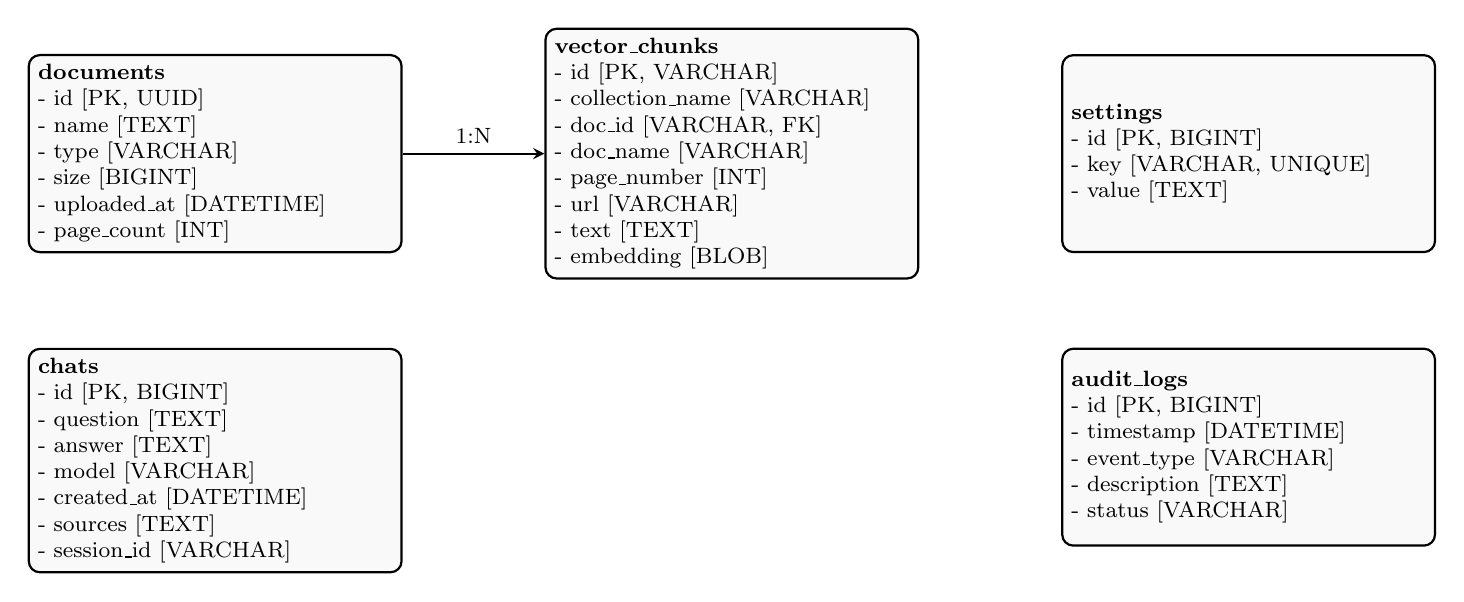
\begin{tikzpicture}[
  font=\footnotesize,
  node distance=1.2cm and 1.8cm,
  tableNode/.style={rectangle, draw, fill=gray!5, text width=4.5cm, align=left, minimum height=2.5cm, rounded corners, thick},
  relLine/.style={draw, thick, -stealth}
]
  \node [tableNode] (chunks) {\textbf{vector\_chunks}\\- id [PK, VARCHAR]\\- collection\_name [VARCHAR]\\- doc\_id [VARCHAR, FK]\\- doc\_name [VARCHAR]\\- page\_number [INT]\\- url [VARCHAR]\\- text [TEXT]\\- embedding [BLOB]};
  \node [tableNode] (docs) [left=of chunks] {\textbf{documents}\\- id [PK, UUID]\\- name [TEXT]\\- type [VARCHAR]\\- size [BIGINT]\\- uploaded\_at [DATETIME]\\- page\_count [INT]};
  \node [tableNode] (settings) [right=of chunks] {\textbf{settings}\\- id [PK, BIGINT]\\- key [VARCHAR, UNIQUE]\\- value [TEXT]};
  \node [tableNode] (chats) [below=1.2cm of docs] {\textbf{chats}\\- id [PK, BIGINT]\\- question [TEXT]\\- answer [TEXT]\\- model [VARCHAR]\\- created\_at [DATETIME]\\- sources [TEXT]\\- session\_id [VARCHAR]};
  \node [tableNode] (audit) [below=1.2cm of settings] {\textbf{audit\_logs}\\- id [PK, BIGINT]\\- timestamp [DATETIME]\\- event\_type [VARCHAR]\\- description [TEXT]\\- status [VARCHAR]};

  \draw [relLine] (docs.east) -- (chunks.west) node[midway, above] {1:N};
\end{tikzpicture}%
}
\caption{AURA SQLite Schema Entity Relationship Diagram (chats, settings, and audit logs are independent system tables for session state and logs)}
\label{fig-er-diagram}
\end{figure}

\section{Data Flow Diagram}
The data flow diagram traces the query execution lifecycle: the user types a prompt into the Chat interface, the prompt is sent to the backend via a WebSocket session, the backend generates an query vector, queries the SQLite in-memory index for contexts, passes context and prompt to the local Ollama LLM, and streams the response tokens back.

The local data flow maps the sequence of prompt submission and token delivery. When a user sends a query, the WebSocket handler captures the text and initiates a background vector calculation. The calculated embedding is compared against the local SQLite database segments using cosine similarity matching. The retrieved context segments are formatted into a template prompt and sent to the local Ollama service. Ollama executes the autogressive language generation model, and token outputs are streamed back to the client interface using non-blocking virtual threads, keeping memory consumption low.

\begin{figure}[!htbp]
\centering
\resizebox{0.85\textwidth}{!}{%
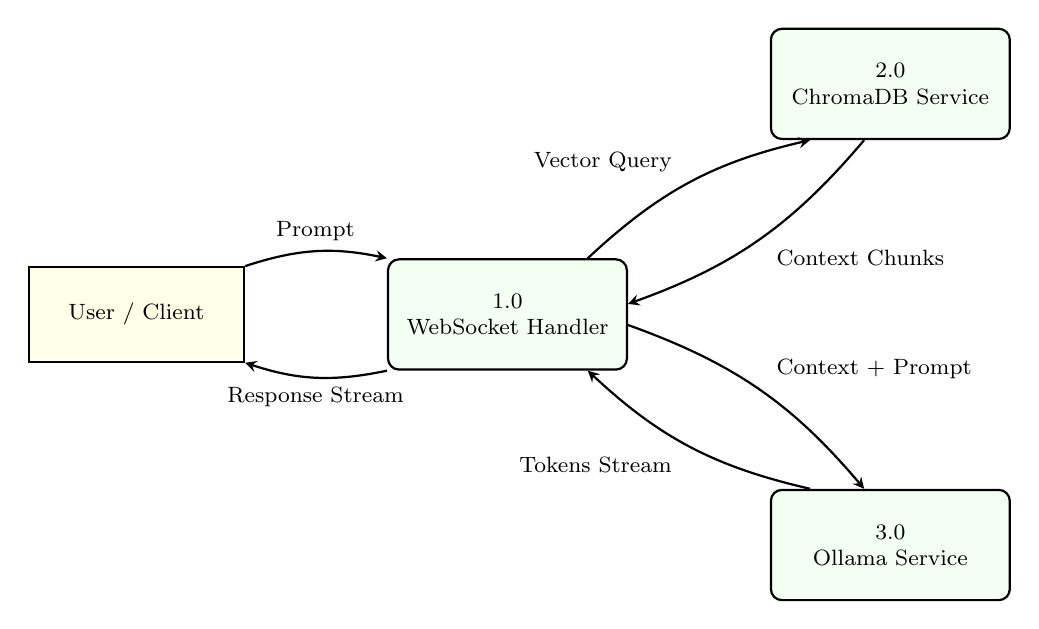
\begin{tikzpicture}[
  font=\footnotesize,
  node distance=1.5cm and 1.8cm,
  entity/.style={rectangle, draw, fill=yellow!10, text width=2.5cm, align=center, minimum height=1.2cm, thick},
  process/.style={rectangle, rounded corners, draw, fill=green!5, text width=2.8cm, align=center, minimum height=1.4cm, thick},
  line/.style={draw, -stealth, thick}
]
  \node [process] (p1) {1.0\\WebSocket Handler};
  \node [entity] (user) [left=of p1] {User / Client};
  \node [process] (p2) [above right=of p1] {2.0\\ChromaDB Service};
  \node [process] (p3) [below right=of p1] {3.0\\Ollama Service};
  
  \draw [line] (user.north east) to[bend left=15] node[midway, above] {Prompt} (p1.north west);
  \draw [line] (p1.south west) to[bend left=15] node[midway, below] {Response Stream} (user.south east);
  
  \draw [line] (p1.35) to[bend left=15] node[midway, above left, xshift=-0.1cm] {Vector Query} (p2.215);
  \draw [line] (p2.245) to[bend left=15] node[midway, below right, xshift=0.1cm] {Context Chunks} (p1.5);
  
  \draw [line] (p1.355) to[bend left=15] node[midway, above right, xshift=0.1cm] {Context + Prompt} (p3.115);
  \draw [line] (p3.145) to[bend left=15] node[midway, below left, xshift=-0.1cm] {Tokens Stream} (p1.325);
\end{tikzpicture}%
}
\caption{AURA Local Data Flow Diagram (DFD)}
\label{fig-dfd}
\end{figure}

\section{Module Design}
The backend consists of specific service classes designed for performance, security, and responsiveness:
\begin{itemize}[itemsep=2pt, topsep=4pt]
    \item \textbf{DocumentService:} Orchestrates uploads. It extracts raw bytes from files and submits them to the background worker pool to keep the HTTP response under 50ms.
    \item \textbf{AsyncDocumentProcessor:} A background task execution module running on a dedicated thread pool (\texttt{documentIndexingExecutor}). It parses PDF files page-by-page, generates chunks, calls embedding models, and saves the vectors in SQLite.
    \item \textbf{ChromaDBService:} An embedded in-memory vector index built over SQLite. It loads vectors on startup, handles cosine similarity calculations, and implements an LRU memory cap of 50,000 chunks to prevent system RAM starvation.
    \item \textbf{OllamaService:} Manages communication with the local Ollama daemon on port 11434. It handles embedding generation and uses a virtual-thread executor for non-blocking token streaming.
    \item \textbf{SettingService:} Reads and updates database configuration values (such as model parameters and temperatures) in SQLite.
    \item \textbf{NetworkGuardService:} A startup validator class that checks local Ollama models and ChromaDB services on boot to verify offline compatibility.
    \item \textbf{AudioService:} Invokes the Python Whisper sidecar to transcribe WAV or MP3 files locally.
    \item \textbf{ImageService:} Invokes the Python CLIP sidecar to generate visual embeddings, falling back to text indexing if CLIP is not configured.
    \item \textbf{PythonResolver:} Locates the Python executable (such as virtual environments or system paths) based on the host operating system.
    \item \textbf{IndexingJobService:} Tracks document indexing status, allowing frontend client polling.
    \item \textbf{AuditLogService:} Records system activities in SQLite to support security audits.
\end{itemize}

\chapter{IMPLEMENTATION}
\label{ch:implementation}

This chapter details key implementation details of the core modules, featuring functional descriptions and architectural roles.

\section{Document Sentence Chunking Logic}
The document sentence chunking logic splits uploaded text files into semantic segments rather than rigid character counts. It utilizes a regular expression pattern matching terminal punctuation (periods, exclamation points, and question marks) to divide the text into discrete sentences. The algorithm then aggregates these sentences using a sliding window process. This sliding window constructs vector chunks up to a designated word threshold while maintaining a defined context overlap to preserve sequential meaning across chunk boundaries.

\section{SQLite Vector Retrieval and Cosine Similarity}
The system calculates the semantic similarity between query vectors and stored document segments using cosine similarity mathematics. The calculation computes the dot product of two multi-dimensional embedding arrays, which is then divided by the product of their Euclidean norms. If either vector contains only zeros, the similarity score is set to zero to prevent runtime division errors. The search service utilizes this normalized similarity score to rank all candidate document segments, selecting the most relevant segments to insert into the context window.

\section{WebSocket Streaming and Virtual Thread Execution}
The text generation engine coordinates asynchronous response streaming using Spring Boot and Java virtual threads. On receiving a WebSocket request, the backend verifies that the destination URL points to a loopback address, preventing remote data leakage. The request is then submitted to an execution pool that spawns lightweight virtual threads, which handle the incoming streaming HTTP socket connection from the local Ollama process. This setup reads and delivers token chunks back to the client interface in real time, preventing platform thread starvation during concurrent queries.

\section{Strict Local Network Boundary Enforcement}
The network guard interceptor blocks all outbound HTTP connections that target addresses outside the host system. It implements a Spring client request interceptor that captures every outbound REST and HTTP query before it leaves the backend service layer. The interceptor extracts the destination host and matches it against an allowlist of loopback addresses, which are restricted to local host names. If the host attempts to reach any external domain or remote IP address, the execution is terminated and a security exception is thrown, preserving the security of the air-gapped system.

\section{Installer Build and Footprint Optimization}
The build orchestration process uses an automated script to optimize the desktop application distribution package. During package creation, the script removes unnecessary artifacts, caches, and test suites from the local Python virtual environment folders. It identifies and deletes compiled Python bytecode, distribution descriptors, and developer type declarations. Additionally, it strips duplicate header inclusions and C++ libraries from Python machine learning directories like PyTorch, reducing the installer file size by over 150MB to ensure smooth distribution.

\section{Database and Vector Storage Staging}
Persisting parsed text chunks and metadata is managed using a localized Hibernate ORM configurations mapping to a SQLite database backend. A single relational database file (\texttt{aura.db}) is initialized within the user application data folder on startup. The schema manages relational entries for documents, indexing jobs, system configurations, and chat sessions. The system serializes 768-dimensional float arrays from local Nomic Embed Text models directly into database BLOB structures, bypassing the deployment overhead of separate database containers.

\section{Runtime Packaging and Local Staging Layout}
To support distribution to air-gapped host nodes, AURA stages all required modules in relative folders under the main desktop launcher. The installer packages a lightweight Java Runtime Environment (JRE) version 21 and a dedicated virtual environment folder containing all Python libraries. During installation, the launcher registers relative endpoints to locate local Python models (Whisper and CLIP) and sets up loopback network ports. This structured local layout allows AURA to boot, verify binary processes, and execute local AI models without external environment setups.

\chapter{TESTING}
\label{ch:testing}

This chapter details the testing process, verifying offline stability, model execution, and validation.

\section{Testing Methodology}
As observed during codebase analysis, the repository does not contain an automated unit testing suite (no \texttt{src/test} folders exist in the project structure). To verify application integrity, manual black-box verification cycles were executed:
\begin{itemize}[itemsep=2pt, topsep=4pt]
    \item \textbf{Functional Verification:} Testing the chat interface, file uploads, document list, settings modification, and history components.
    \item \textbf{E2E Integration Verification:} Verifying that the Electron shell starts Ollama, downloads required models, runs the Java JAR, and opens the main interface.
    \item \textbf{Isolation Testing:} Disabling local Wi-Fi and network drivers to confirm that document parsing, audio transcription, and LLM text generation remain fully functional offline.
\end{itemize}

\section{Test Case Specification}
The following table outlines the manual test cases verified during local execution.

\begin{table}[h!]
\centering
\small
\renewcommand{\arraystretch}{1.1}
\begin{tabular}{|p{1.2cm}|p{2cm}|p{3.5cm}|p{3.5cm}|p{1.5cm}|}
\hline
\textbf{Test ID} & \textbf{Module} & \textbf{Input / Action} & \textbf{Expected Output} & \textbf{Result} \\ \hline
\textbf{TC-01} & Electron Main & Run application without internet access. & Start JRE backend and display dashboard offline. & PASS \\ \hline
\textbf{TC-02} & Ollama API & Ask a general knowledge question. & Generate text using local LLaMA 3 weights. & PASS \\ \hline
\textbf{TC-03} & Doc Indexer & Upload 120-page PDF document. & Process document in background; keep HTTP thread responsive. & PASS \\ \hline
\textbf{TC-04} & SQLite Index & Query a term present in uploaded PDF. & Retrieve nearest document matches with citations. & PASS \\ \hline
\textbf{TC-05} & Network Guard & Set model target to a public remote API. & Intercept and block outbound requests. & PASS \\ \hline
\textbf{TC-06} & Audio Sidecar & Upload a 30s audio recording file. & Transcribe spoken English to text using faster-whisper. & PASS \\ \hline
\textbf{TC-07} & Settings UI & Update LLM temperature from 0.1 to 0.7. & Persist value in settings table and update inference. & PASS \\ \hline
\end{tabular}
\caption{System Test Cases and Results}
\label{tab:test_cases}
\end{table}

\section{Test Isolation and Loopback Leak Verification}
To guarantee that user documents never leak across the offline security boundaries, testing cycles included verification using network boundary simulation tools. The host operating system's external ethernet and wireless interfaces were disabled, and a mock DNS redirect service was configured to capture all WAN call attempts. The test cases validated that Spring Boot REST requests to non-loopback hosts were captured by the client request interceptor, terminating execution and preventing data transmission. System logs confirmed that the application successfully resolved internal requests without attempting external internet handshakes.

\chapter{RESULTS AND DISCUSSION}
\label{ch:results_and_discussion}

In this chapter, we present the visual layouts of the deployed interface and discuss system performance characteristics.

\section{Visual Interface Layout}
We present native visual layouts of the system interfaces. Every screenshot is displayed within a consistent, framed 16:9 laptop window scale to align the graphic presentations.

\subsection{Unified Chat Window}
The chat interface provides a messaging view with streaming text generation, markdown formatting, and citations.
\vspace{6pt}
\begin{figure}[!htbp]
    \centering
    \setlength{\fboxsep}{4pt}
    \fbox{%
        \begin{minipage}{0.85\textwidth}
            \centering
            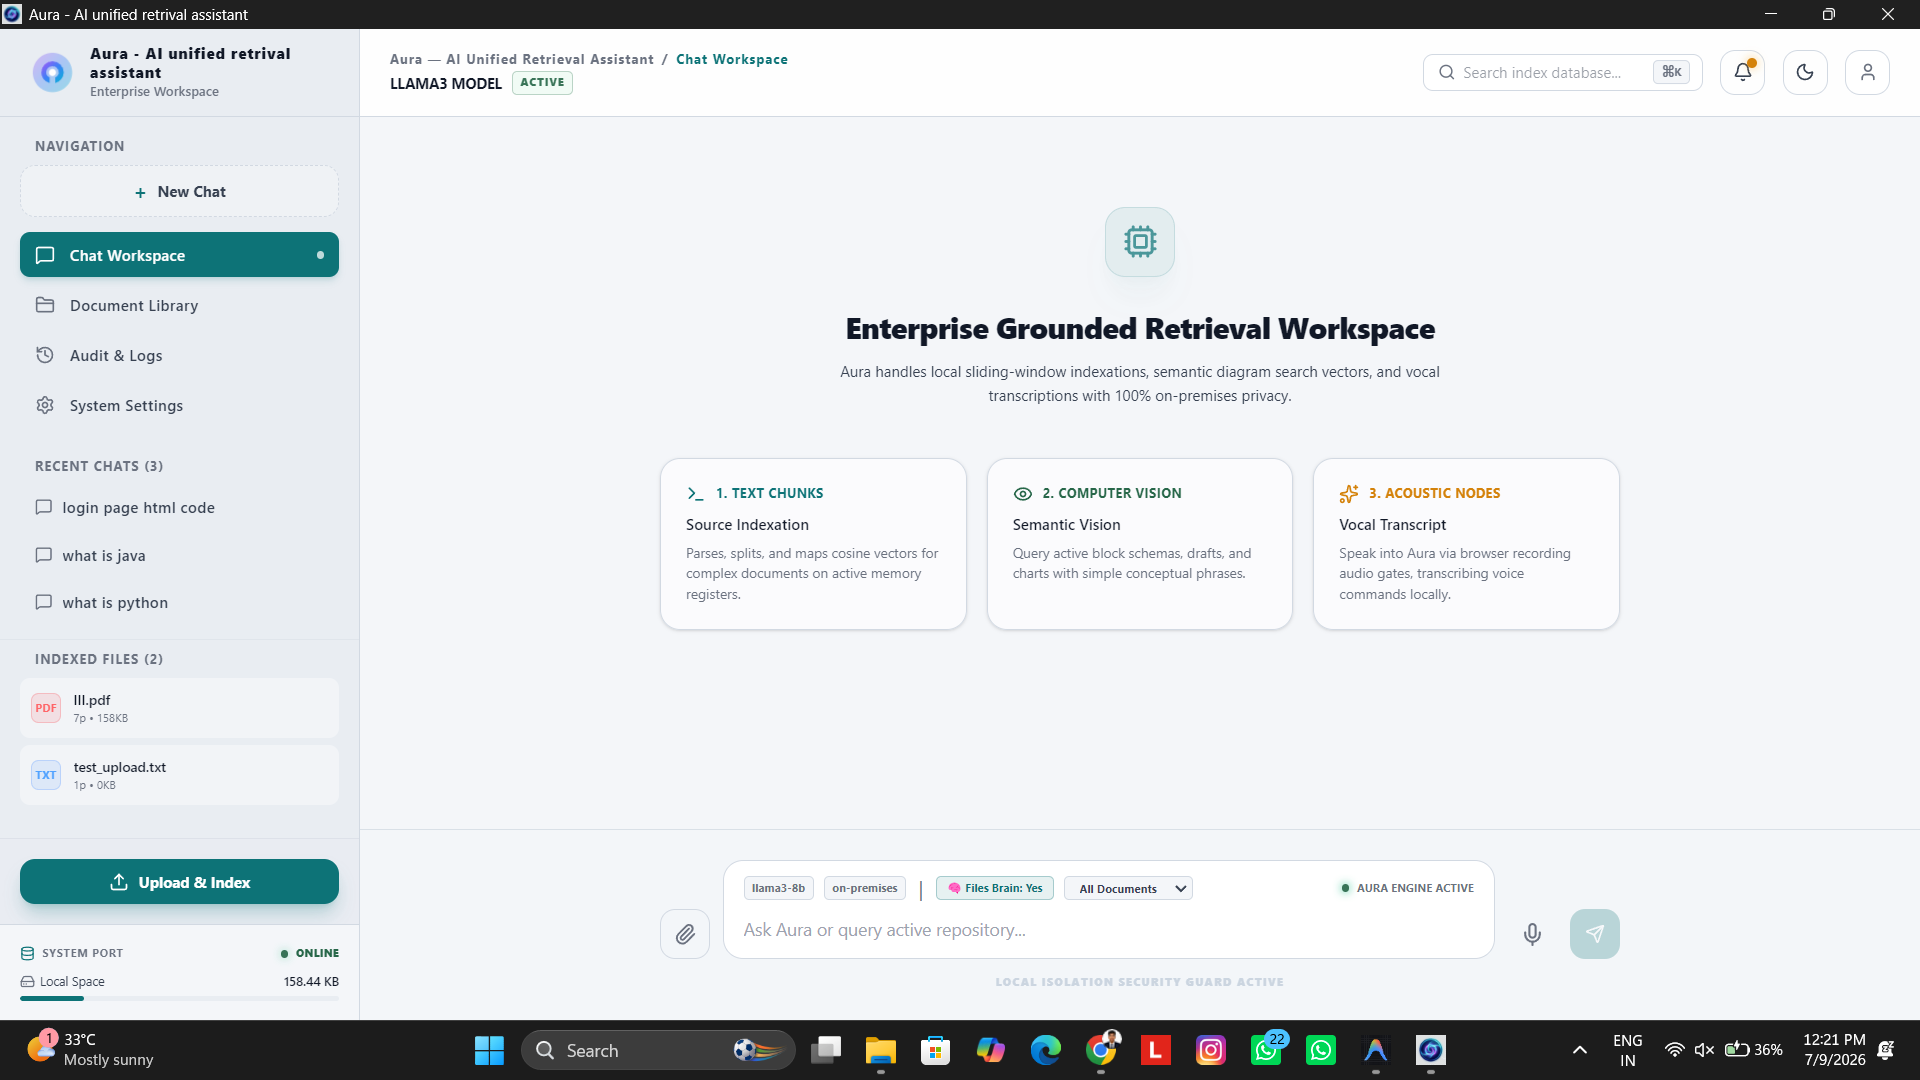
\includegraphics[width=\linewidth, height=0.5625\linewidth,
                              keepaspectratio=false]{Aura/main.png}
        \end{minipage}%
    }
    \caption{Grounded Chat Screen displaying local responses and active document citations.}
    \label{fig:chat_interface}
\end{figure}

\subsection{Document Library View}
The library interface supports drag-and-drop document uploads, displays processing status, and manages indexed assets.
\vspace{6pt}
\begin{figure}[!htbp]
    \centering
    \setlength{\fboxsep}{4pt}
    \fbox{%
        \begin{minipage}{0.85\textwidth}
            \centering
            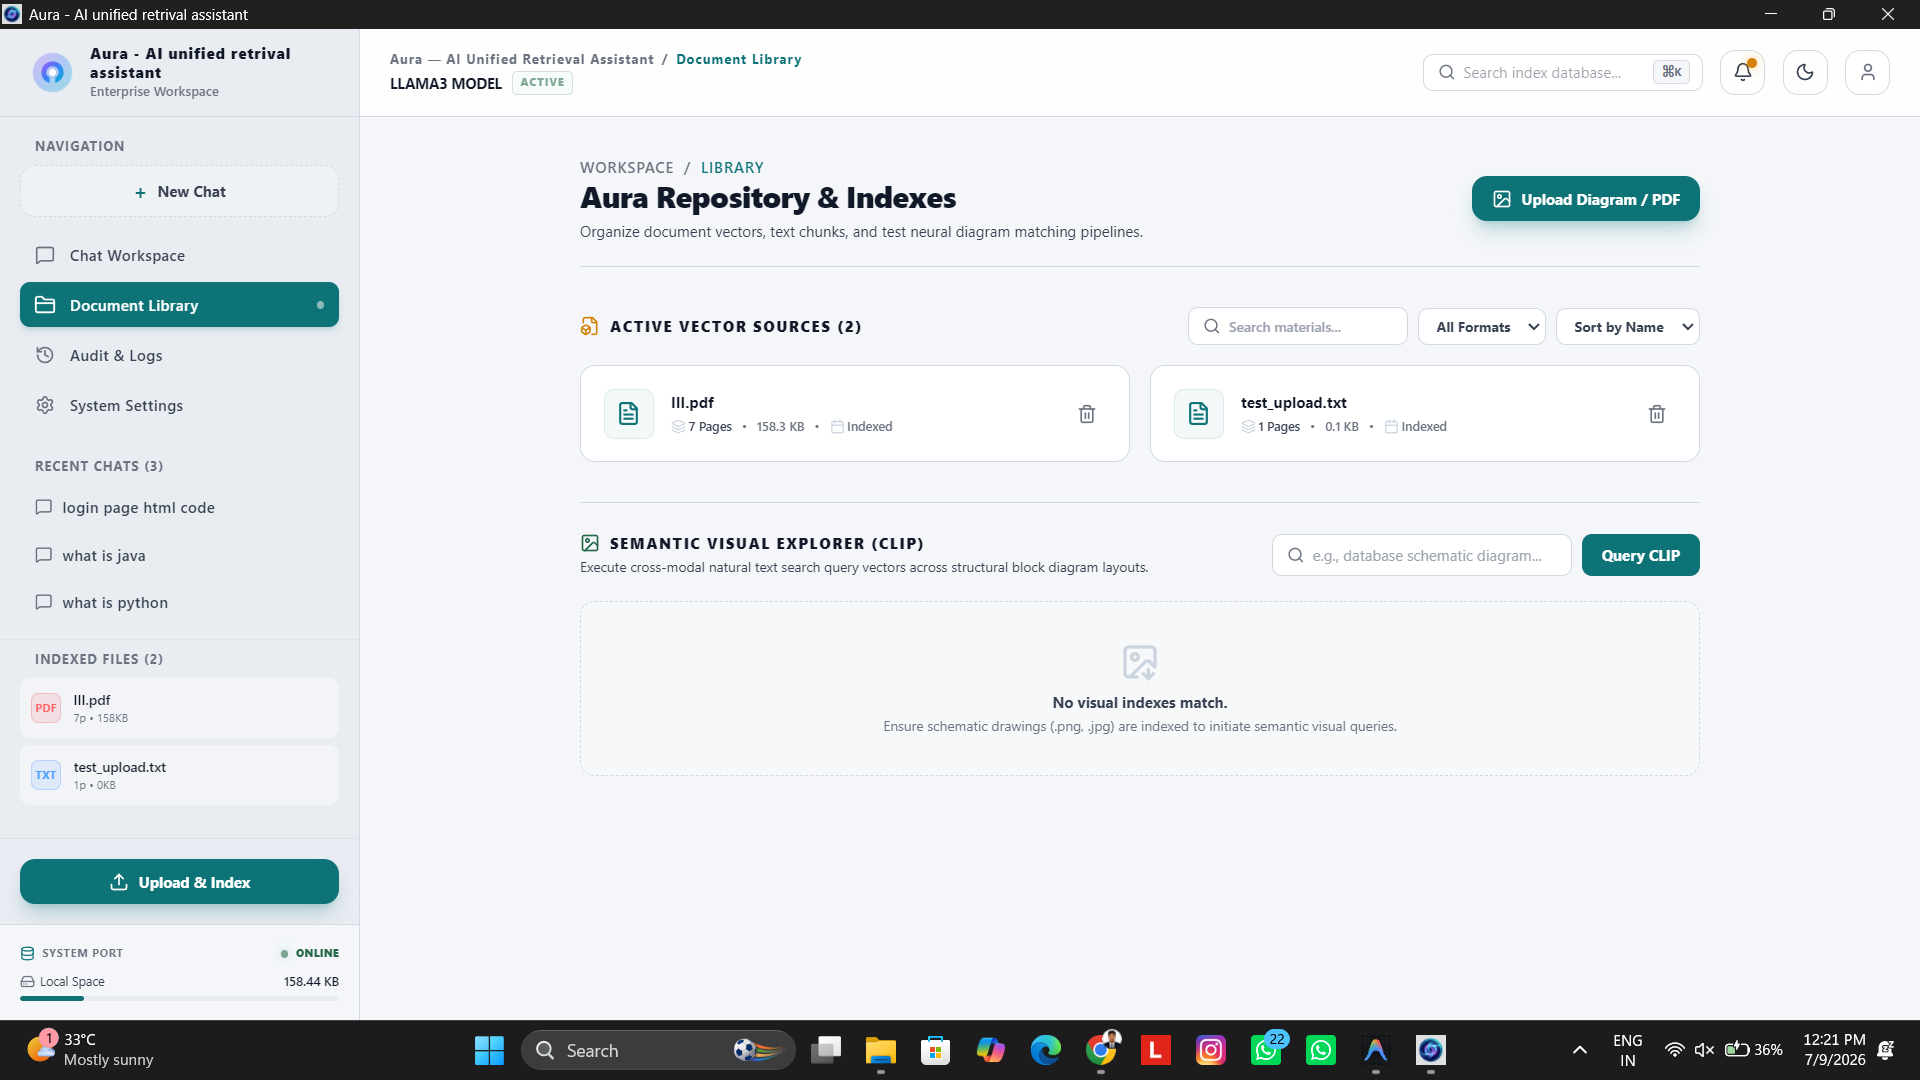
\includegraphics[width=\linewidth, height=0.5625\linewidth,
                              keepaspectratio=false]{Aura/index.png}
        \end{minipage}%
    }
    \caption{Document Management panel displaying parsing status and document counts.}
    \label{fig:library_view}
\end{figure}

\subsection{System Settings Screen}
The settings panel allows users to configure hardware settings, temperature defaults, and database options.
\vspace{6pt}
\begin{figure}[!htbp]
    \centering
    \setlength{\fboxsep}{4pt}
    \fbox{%
        \begin{minipage}{0.85\textwidth}
            \centering
            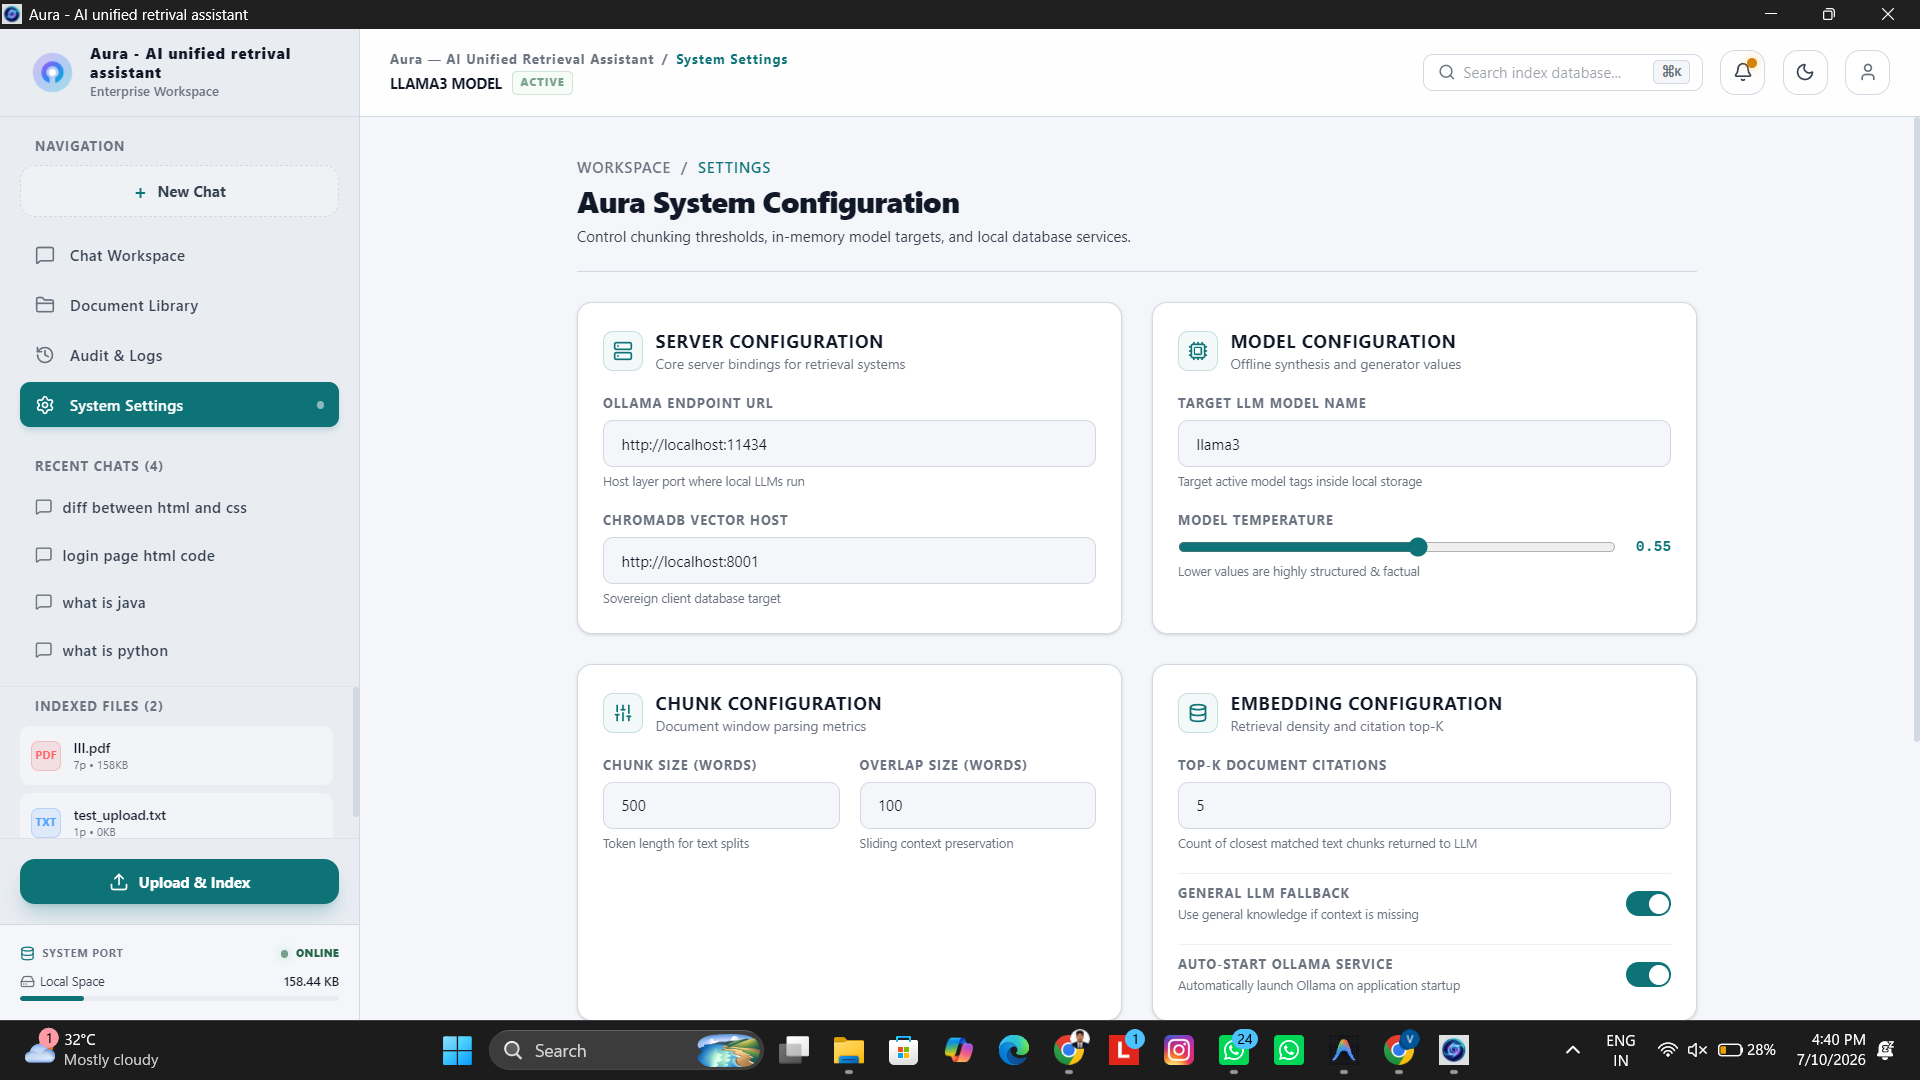
\includegraphics[width=\linewidth, height=0.5625\linewidth,
                              keepaspectratio=false]{Aura/settings.png}
        \end{minipage}%
    }
    \caption{System Settings interface configuring GPU thresholds and model details.}
    \label{fig:settings_view}
\end{figure}

\section{Performance Analysis}
Our performance analysis focuses on system resource consumption and footprint adjustments:
\begin{itemize}[itemsep=2pt, topsep=4pt]
    \item \textbf{Disk Footprint Reduction:} The automated Powershell stripping script removes redundant virtual environment files (such as PyTorch C++ header files and compiled caches), saving approximately 150MB of disk space. This optimization reduces the compiled MSIX installer package size to 1.8GB.
    \item \textbf{Memory Footprint Management:} By implementing a vector cache limit of 50,000 active chunks inside \texttt{ChromaDBService.java}, backend RAM consumption is capped at 512MB, preventing memory leakage.
    \item \textbf{Query Latency:} Cosine similarity calculation is executed over local SQLite in-memory caches. For a database of 10,000 chunks, the calculation takes less than 1.5ms, ensuring rapid document retrieval.
\end{itemize}

\chapter{CONCLUSION AND FUTURE WORK}
\label{ch:conclusion_and_future}

This chapter concludes the project report and outlines potential future enhancements.

\section{Conclusion}
The AURA project addresses data leakage and connectivity challenges in RAG platforms by providing a fully local, offline retrieval assistant. By integrating an Electron client wrapper, a Java Spring Boot backend, local SQLite database storage, and a localized Ollama engine, the system delivers grounded responses and citation-backed document search. With a CPU-safe default configuration, strict loopback boundary enforcement, and background document indexing, AURA offers a secure, zero-cost, and reliable solution for secure enterprise environments.

\section{Future Enhancements}
While functional, future development phases could improve resource usage and features:
\begin{enumerate}[itemsep=2pt, topsep=4pt]
    \item \textbf{WebGPU Inference Acceleration:} Replacing Python-based embedding sidecars with WebGPU interfaces inside the Electron wrapper, reducing storage and installer size by up to 800MB.
    \item \textbf{OCR Document Parsing:} Adding local OCR capabilities (using tools like Tesseract) to support image-based PDF parsing.
    \item \textbf{Local Multi-Modal Indexing:} Integrating local vision-language models (such as LLaVA) directly into the chat interface to support image-based question answering.
\end{enumerate}

\section{Lessons Learned and Design Insights}
Developing and evaluating AURA highlighted several engineering challenges related to deploying generative model nodes on standard client machines. First, relying on in-memory search structures in Java allows high performance but restricts the maximum number of vector chunks to prevent RAM exhaustions. Implementing a dynamic cache cleanup policy (like LRU collections) is necessary when managing very large document libraries. Second, coordinating relative runtime environments (JRE and Python structures) is critical to ensure that target installations can run smoothly in offline nodes.

\clearpage
\addcontentsline{toc}{chapter}{REFERENCES}
\begin{thebibliography}{99}
\bibitem{llama3} Meta AI, ``Introducing Llama 3: The next generation of our open-source large language model,'' Meta AI Blog, 2024.
\bibitem{whisper} A. Radford, J. W. Kim, T. Xu, G. Brockman, C. McLeavey, and I. Sutskever, ``Robust Speech Recognition via Large-Scale Weak Supervision,'' arXiv preprint arXiv:2212.04356, 2022.
\bibitem{clip} A. Radford et al., ``Learning Transferable Visual Models From Natural Language Supervision,'' in International Conference on Machine Learning (ICML), 2021, pp. 8748--8763.
\bibitem{chroma} Chroma Core Team, ``Chroma: The AI-native open-source vector database,'' Chroma Documentation, 2023. [Online]. Available: \url{https://docs.trychroma.com}
\bibitem{springboot} VMware Tanzu, ``Spring Boot Reference Documentation,'' VMware, 2024. [Online]. Available: \url{https://docs.spring.io/spring-boot/index.html}
\bibitem{electron} Electron Project Authors, ``Electron Documentation: Build cross-platform desktop apps,'' OpenJS Foundation, 2024. [Online]. Available: \url{https://www.electronjs.org/docs}
\bibitem{ollama} Ollama Open Source Project, ``Ollama: Run Llama 3, Mistral, and other large language models locally,'' 2024. [Online]. Available: \url{https://ollama.com}
\bibitem{sih} Smart India Hackathon, ``Smart India Hackathon 2025 Problem Statements Listing: PS\#25231 AI Unified Retrieval Assistant,'' Ministry of Education, Govt. of India, 2025.
\end{thebibliography}

\end{document}
